\documentclass[10pt]{beamer}               % only frames
%\documentclass[10pt, notes]{beamer}       % print frame + notes
%\documentclass[10pt, notes=only]{beamer}   % only notes

\usetheme[numbering=fraction]{metropolis}
\usepackage{appendixnumberbeamer}

\usepackage{booktabs}
\usepackage[scale=2]{ccicons}

\usepackage{pgfplots}
\usepgfplotslibrary{dateplot}

\usepackage{xspace}
\newcommand{\themename}{\textbf{\textsc{metropolis}}\xspace}

% Defining Imperial colors
\definecolor{ImpDB}{HTML}{003E74}
\definecolor{ImpLB}{HTML}{EB811B} % orange color EB811B replaced by Imperial light blue
\definecolor{ImpNavy}{HTML}{002147}
\definecolor{AlertRed}{HTML}{E22012}%{92140C}E22012
\definecolor{ExampleGreen}{HTML}{036D19}

\setbeamercolor{progress bar}{fg=ImpDB}
\setbeamercolor{frametitle}{bg=ImpDB}
\setbeamercolor{alerted text}{fg=AlertRed}
%\setbeamercolor{block title alert}{fg=AlertRed, bg=AlertRed!40!white} 
\setbeamercolor{block title example}{fg=ExampleGreen} %bg=ExampleGreen!40!white 
\setbeamercolor{palette primary}{fg=white, bg=ImpDB} % Corrects standout slides

\usepackage{verbatim}

\DeclareMathOperator*{\argmin}{arg\,min}
\DeclareMathOperator*{\argmax}{arg\,max}
\usepackage{bm}
%=========================================================
% Presentation specific fields below here
%=========================================================

\title{Inference for Extreme Earthquake Magnitudes}
\subtitle{How to use and learn from small seismic events}
\date{$M_{\text{max}}$ Workshop, June 2022.}
\author{\textbf{Zak Varty}, Jonathan Tawn, Peter Atkinson \& Stijn Bierman}
\institute{Lancaster University, Shell}

\setbeamertemplate{frame footer}{\textbf{Z Varty}, J Tawn, P Atkinson \& S Bierman. Inference for Extreme Earthquake Magnitudes}

% Left aligned title logo
%\titlegraphic{
%\hfill  % uncomment to right-align logo
%
\includegraphics[width = %3.5cm]{Imperial_1_Pantone_solid.eps}
%}



% Uncomment to add logo to each slide
%\logo{
%
\includegraphics[width = 2cm]{Imperial_1_Pantone_solid.eps}
%}

\setbeamercolor{background canvas}{bg=white}




\begin{document}

\maketitle

\begin{frame}{Where am I going with all this?}
\textbf{Part 1:} Why care about teaching ethics?

\vspace{2em}

\textbf{Part 2:} A bit of context 

\vspace{2em}

\textbf{Part 3:} 5 Principles (+ \underline{Tips}!)

\vspace{2em}

\textbf{Part 4:} Action.
\end{frame}

\section{Why should you care about teaching ethics?}

\begin{frame}{Data Science: Miracle Cure and Sexiest job}
 
 \begin{columns}
 \begin{column}{0.4\textwidth}
 \begin{itemize}
     \item Healthcare 
     \item []
     \item Ecology \& Conservation 
     \item []
     \item Business \& Government 
     \item []
     \item Environment
 \end{itemize}
 \end{column}
 \begin{column}{0.6\textwidth}
    \centering
    \vspace{2em}
    \\
    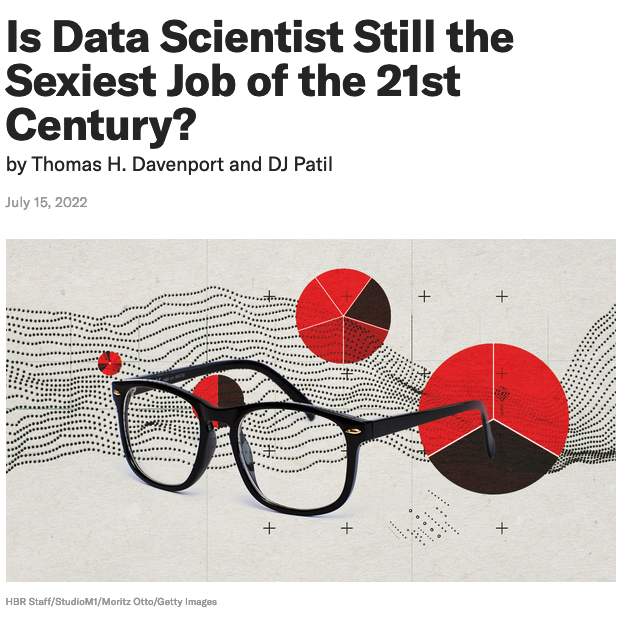
\includegraphics[width = 0.55\textwidth]{images/Screenshot 2022-08-31 at 11.29.17.png}
    \\
    \footnotesize{\textbf{Source:} Harvard Business Review}
 \end{column}
 \end{columns}
\end{frame} 

\begin{frame}{Data Science: What could possibly go wrong?}
 \begin{columns}
 \begin{column}{0.5\textwidth}
    \centering
    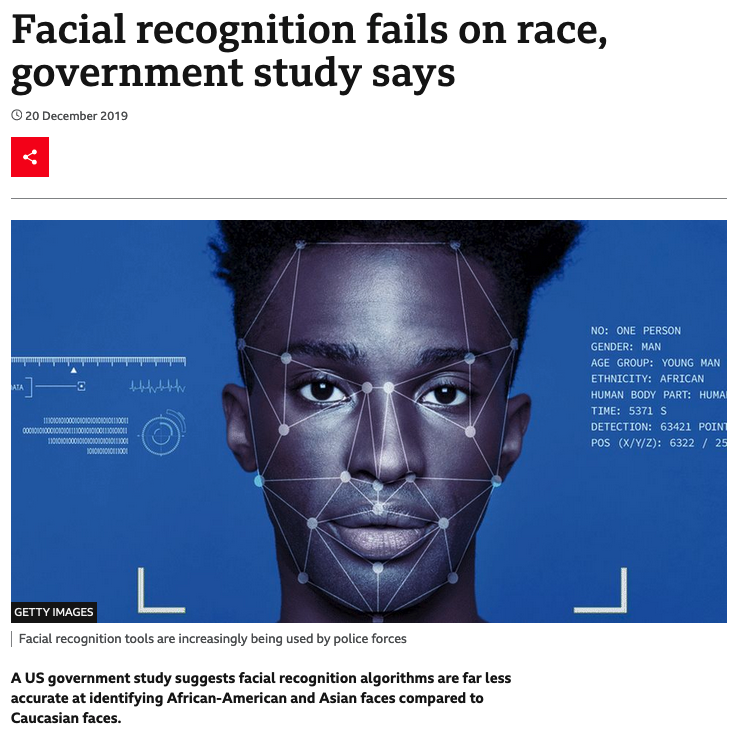
\includegraphics[width = 0.7\textwidth]{images/bbc-facial-recognition.png}
 \end{column}
 \begin{column}{0.5\textwidth}
    \centering
    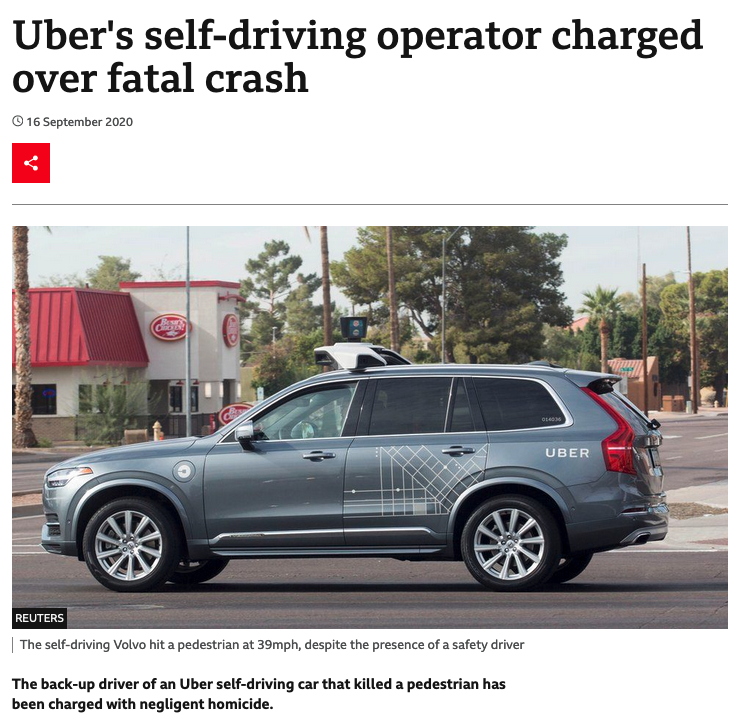
\includegraphics[width = 0.7\textwidth]{images/bbc-self-driving_1.png}
 \end{column}
 \end{columns}
\end{frame} 

\begin{frame}{Data Science: What could possibly go wrong?}
    \centering
    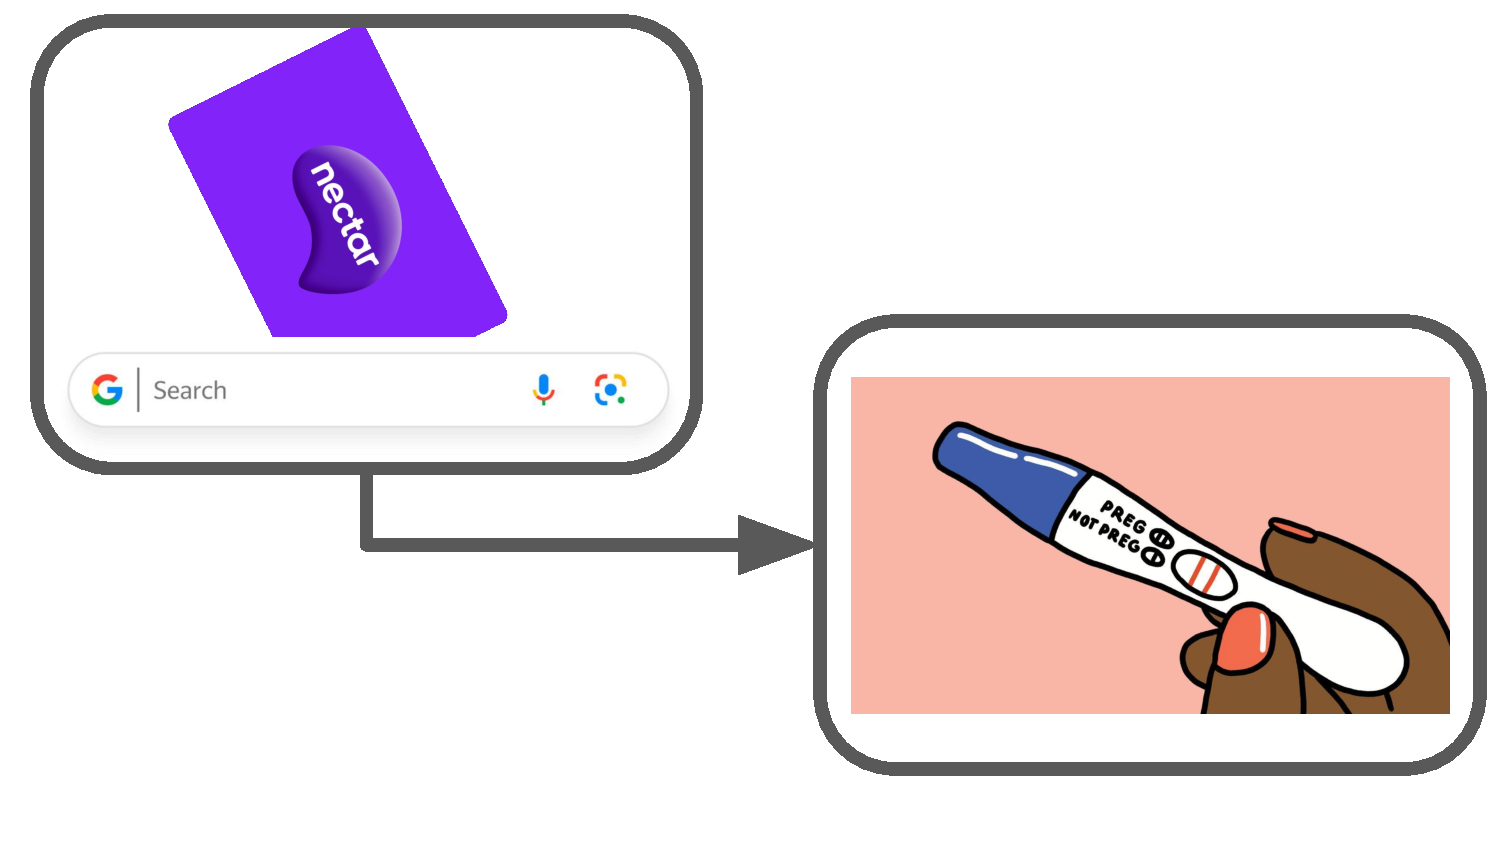
\includegraphics[width = 0.85\textwidth]{images/pregnancy-prediction.pdf}
\end{frame} 

\section{A bit of context}

\begin{frame}{Imperial MSc in Machine Learning and Data Science}
\centering
\includegraphics[width = 0.8\textwidth, page = 2]{images/RSS_pictures.pdf}
\end{frame}

\section{\quad 5 Principles of Ethical DS \\ \large{(+ how you might already teach them)}}

\begin{frame}{Principle 1: Privacy \& Autonomy}
\begin{columns}
    \begin{column}{0.7 \textwidth}
     \includegraphics[width = \textwidth, page = 3]{images/RSS_pictures.pdf}
    \end{column}
    \begin{column}{0.3 \textwidth}
    Privacy and Autonomy
    \end{column}
\end{columns}
\end{frame}

\begin{frame}{Principle 2: Fairness}
\begin{columns}
    \begin{column}{0.3 \textwidth}
    Fairness
    \end{column}
    \begin{column}{0.7 \textwidth}
     \includegraphics[width = \textwidth, page = 4]{images/RSS_pictures.pdf}
    \end{column}
\end{columns}
\end{frame}

\begin{frame}{Principle 3: Value Alignment}
\begin{columns}
    \begin{column}{0.67 \textwidth}
     \includegraphics[width = \textwidth, page = 5]{images/RSS_pictures.pdf}
    \end{column}
    \begin{column}{0.32 \textwidth}
    Value Alignment
    \end{column}
\end{columns}
\end{frame}

\begin{frame}{Principle 4: Explainability \& Interpretability}
\begin{columns}
    \begin{column}{0.3 \textwidth}
    Explainability \& Interpretability
    \end{column}
    \begin{column}{0.7 \textwidth}
     \includegraphics[width = \textwidth, page = 6]{images/RSS_pictures.pdf}
    \end{column}
\end{columns}
\end{frame}

\begin{frame}{Principle 5: Safety, Security and Accountability}
\begin{columns}
    \begin{column}{0.6 \textwidth}
     \includegraphics[width = \textwidth, page = 7]{images/RSS_pictures.pdf}
    \end{column}
    \begin{column}{0.4 \textwidth}
    Value Alignment
    \end{column}
\end{columns}
\end{frame}

\end{document}

